%! Author = Antonio Lobo
%! Date = 30/10/2024

\subsection{Reduction Methods}
In this section, we briefly describe reduction techniques used for instance-based learning, illustrating with simple 2D datasets.

\subsubsection{GCNN}

The Generalized Condensed Nearest Neighbor (GCNN) \cite{chang2006adaptive} algorithm extends the traditional Condensed Nearest Neighbor (CNN) method by incorporating adaptive prototype learning. This \textbf{undersampling} technique seeks a subset of prototypes $U \subseteq X$, where $X = \{(x_1, y_1), \ldots, (x_n, y_n)\}$ is our dataset, that correctly represents the data. This approach is especially beneficial for unbalanced datasets. The main idea behind CNN is to select prototypes that \textit{absorb} points which they can represent as prototypes. The steps for this method are as follows:

\begin{enumerate}
	\item \textbf{Prototype Selection:} For each class $c_j$, let $X_j = \{ (x, y) : y = c_j\}$ be all points of this class. We select as a prototype $x_j^*$, the point that is the nearest neighbor of the most other points in $X_j$. Thus, $x_j^*$ will influence the maximum number of points in any KNN decision. Specifically,
	$$
	x_j^* = \arg\max_{x \in X_j} \left( \sum_{x' \in X_j \setminus \{x\}}\left(x = \operatorname{NN}_{X_j \setminus \{x'\}}(x')\right) \right).
	$$
	Hence, $U = \{ x_j^* : j = 1, \ldots, m \}$ and $U_j$ will denote all prototypes for class $c_j$.
	
	\item \textbf{Absorption:} This step distinguishes GCNN from CNN. Define $\delta_n = \min_{\{ (x_i, y_i), (x_j, y_j) \in X : y_i \neq y_j\}} \left( \|x_i - x_j\| \right)$. For each point $x_i$, let $p = \arg\min_{x \in U_j} \left( ||x - x_i|| \right)$ and $q = \arg\min_{x \in (U \setminus U_j)} \left( ||x - x_i|| \right)$ be the nearest prototypes from the same class and a different class, respectively. We absorb $x_i$ if:
	$$
	\| \mathbf{x} - \mathbf{q} \| - \| \mathbf{x} - \mathbf{p} \| > \rho \delta_n, \quad \rho \in [0, 1).
	$$
	In CNN, $\rho = 0$, meaning $x_i$ is absorbed if its nearest prototype is from its class. The parameter $\rho$ introduces a slack in this decision, illustrated in \textbf{Figure} \ref{fig:gcnnRhoIllustration}.
	
	\begin{figure}[ht]
		\centering
		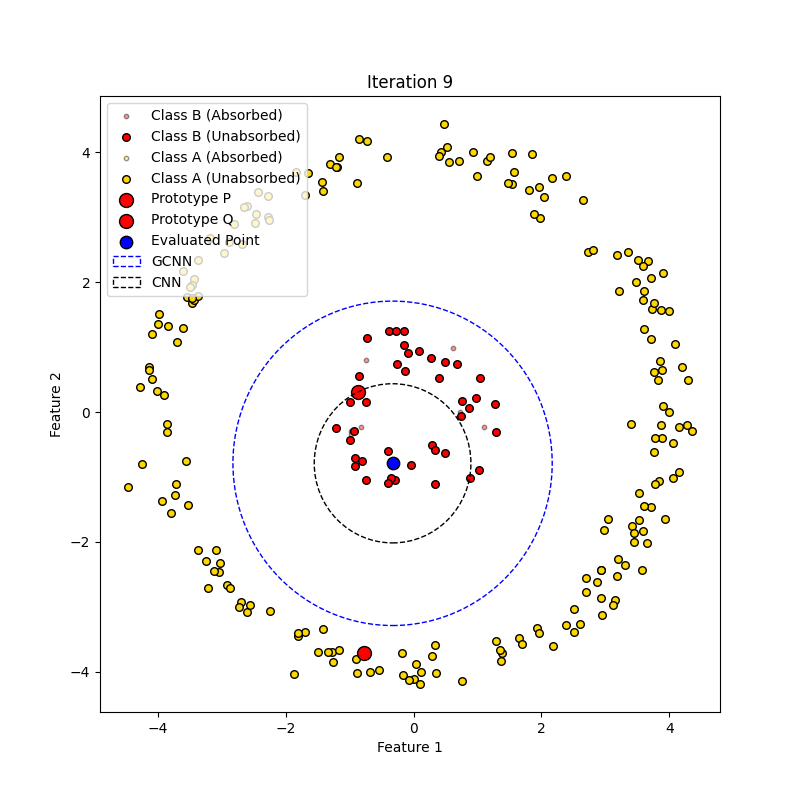
\includegraphics[width=0.4\textwidth]{figures/gcnn/gcnnRhoIllustration}
		\caption{Effect of $\rho$ in GCNN}
		\label{fig:gcnnRhoIllustration}
	\end{figure}
	
	\item \textbf{Prototype Augmentation:} If points remain unabsorbed for class $c_j$, repeat prototype selection on these unabsorbed points, then return to Step 2. The process stops once all points are absorbed.
\end{enumerate}

In \textbf{Figures} \ref{fig:rho_variation_1} and \ref{fig:rho_variation_2}, we illustrate the effects of varying $\rho$ from 0 to 1 on a dataset.

\begin{figure}[ht]
	\centering
	\begin{subfigure}[b]{0.3\textwidth}
		\centering
		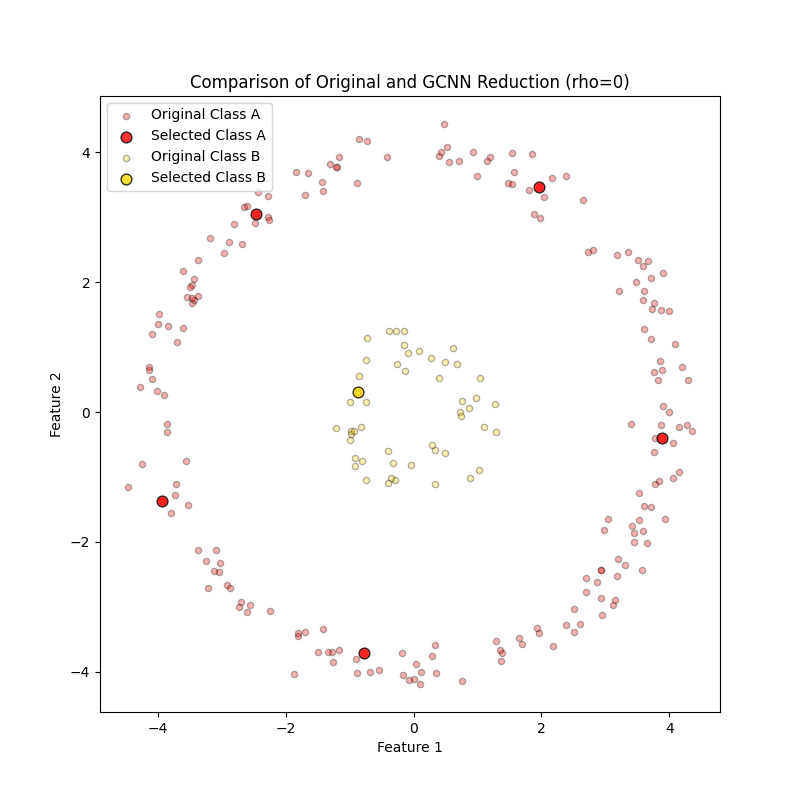
\includegraphics[width=\textwidth]{figures/gcnn/comparison_plot_rho_0.png}
		\caption{$\rho = 0$}
		\label{fig:rho0}
	\end{subfigure}
	\hfill
	\begin{subfigure}[b]{0.3\textwidth}
		\centering
		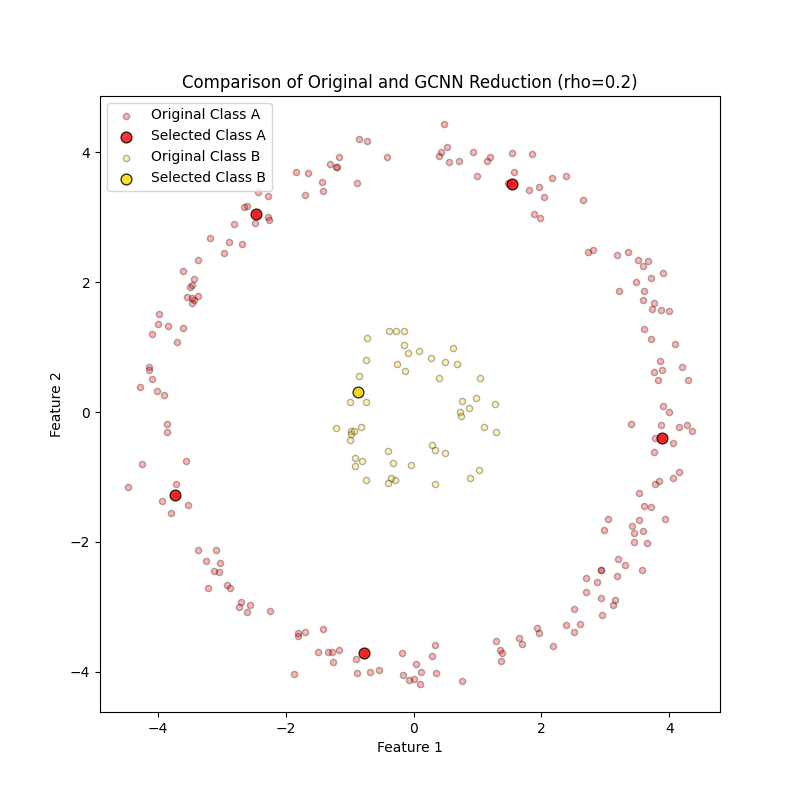
\includegraphics[width=\textwidth]{figures/gcnn/comparison_plot_rho_0.2.png}
		\caption{$\rho = 0.2$}
		\label{fig:rho0.2}
	\end{subfigure}
	\hfill
	\begin{subfigure}[b]{0.3\textwidth}
		\centering
		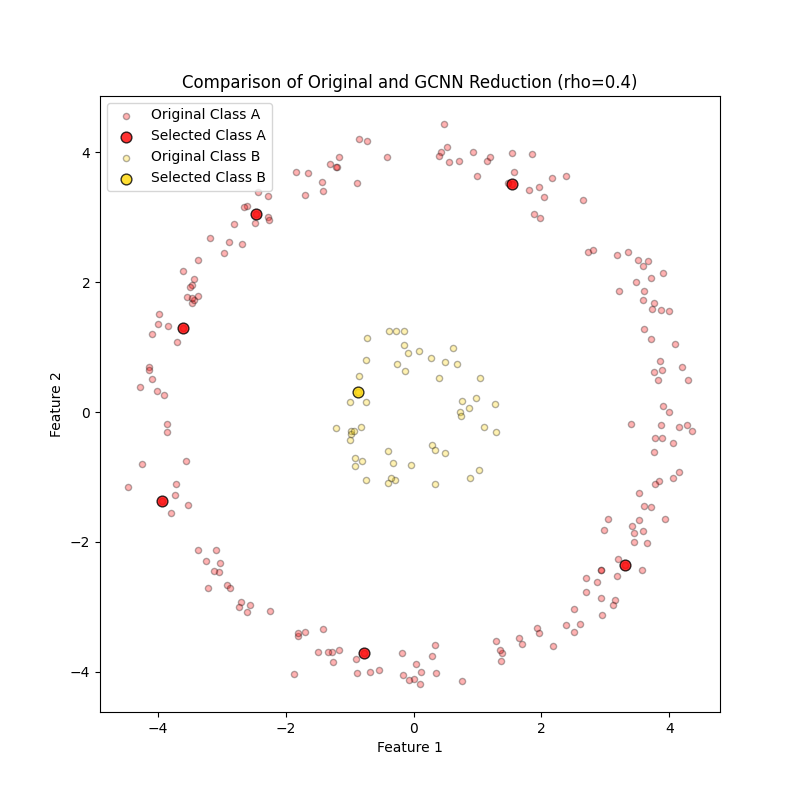
\includegraphics[width=\textwidth]{figures/gcnn/comparison_plot_rho_0.4.png}
		\caption{$\rho = 0.4$}
		\label{fig:rho0.4}
	\end{subfigure}
	\caption{GCNN illustration for $\rho=0, 0.2, 0.4$}
	\label{fig:rho_variation_1}
\end{figure}

\begin{figure}[ht]
	\centering
	\begin{subfigure}[b]{0.3\textwidth}
		\centering
		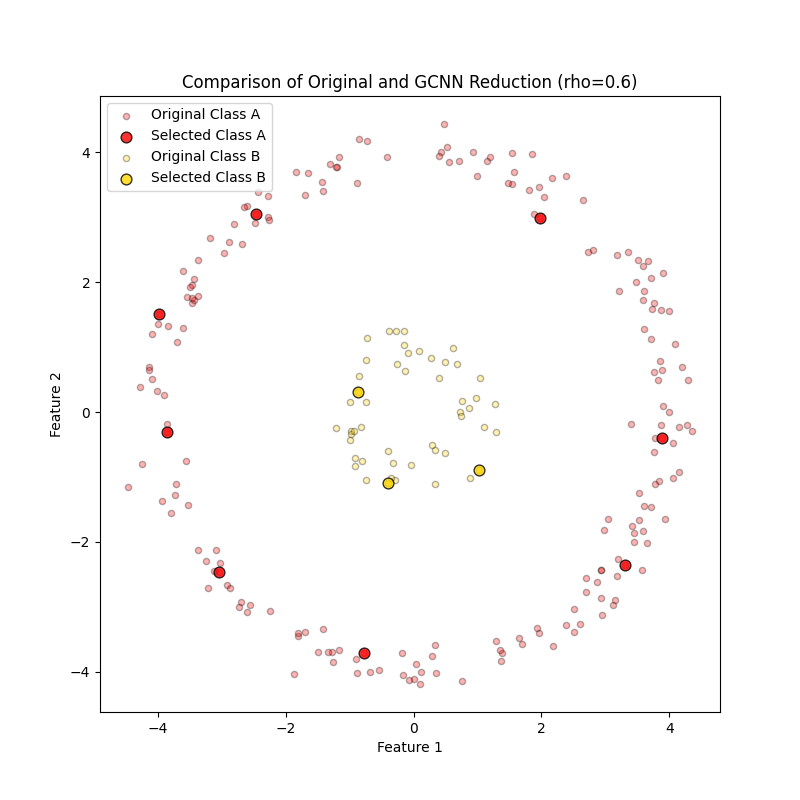
\includegraphics[width=\textwidth]{figures/gcnn/comparison_plot_rho_0.6.png}
		\caption{$\rho = 0.6$}
		\label{fig:rho0.6}
	\end{subfigure}
	\hfill
	\begin{subfigure}[b]{0.3\textwidth}
		\centering
		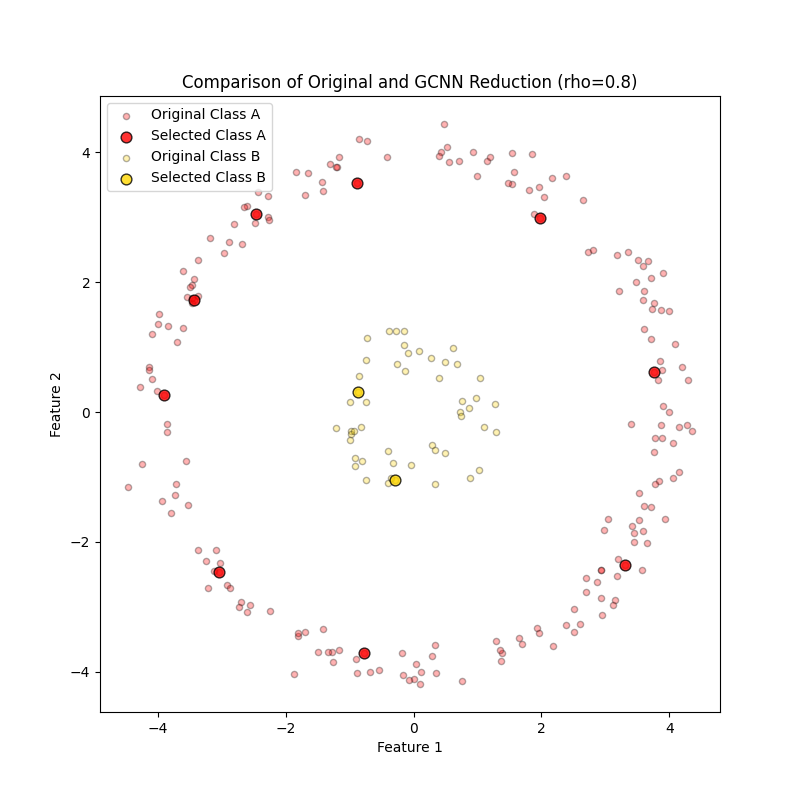
\includegraphics[width=\textwidth]{figures/gcnn/comparison_plot_rho_0.8.png}
		\caption{$\rho = 0.8$}
		\label{fig:rho0.8}
	\end{subfigure}
	\hfill
	\begin{subfigure}[b]{0.3\textwidth}
		\centering
		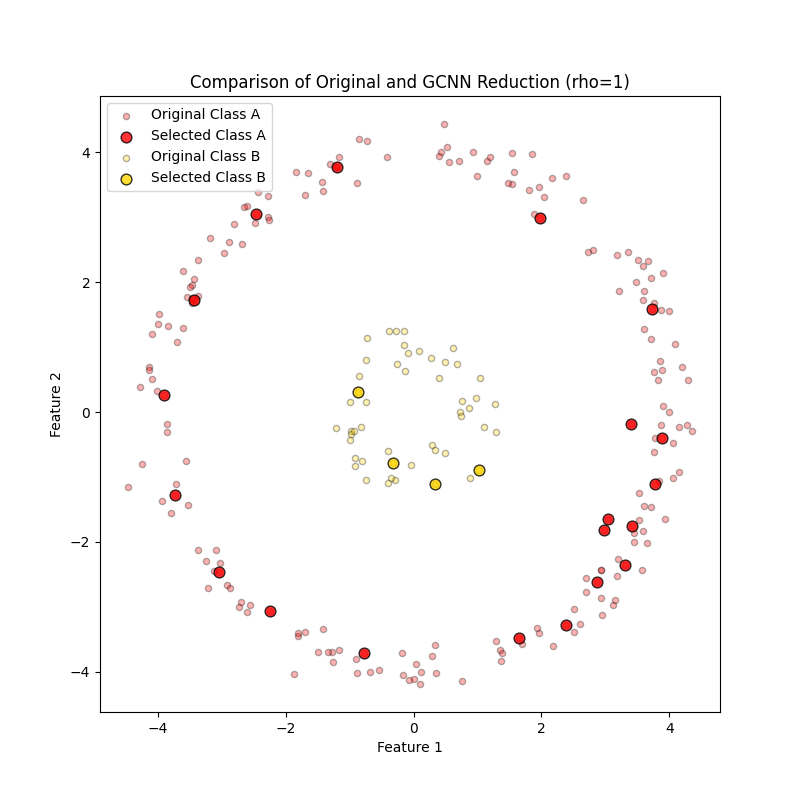
\includegraphics[width=\textwidth]{figures/gcnn/comparison_plot_rho_1.png} % Add the new plot here
		\caption{$\rho = 1$}
		\label{fig:rho1}
	\end{subfigure}
	\caption{GCNN illustration $\rho=0.6,0.8,1$}
	\label{fig:rho_variation_2}
\end{figure}

\subsubsection{EENTH}
This subsection outlines the Elimination Editing with Nearest-neighbor Threshold (EENTH) method \cite{vazquez2005}, which uses a modified $k$-NN rule with probability-based decisions to eliminate instances, particularly useful for noise removal. The main steps are:

\begin{enumerate}
	\item \textbf{Probability-based Classification}: For each instance $x$, calculate the probability $p_i(x)$ of $x$ belonging to class $i$ based on its $k$-nearest neighbors. Probabilities are weighted inversely by distance and normalized:
	\begin{align}
		p_i^j &= \frac{|\{x_k \in NN_k(x) : y_k = j \}|}{k} \\
		P_i(x) &= \sum_{j=1}^{k} p_i^j \frac{1}{1 + d(x, x^j)} \\
		p_i(x) &= \frac{P_i(x)}{\sum_{j=1}^{M} P_j(x)}
	\end{align}
	
	\item \textbf{Thresholding}: Define a threshold $\mu$ to refine classification by identifying instances near decision boundaries where $p(x) < \mu$ as candidates for removal.
	
	\item \textbf{Elimination}: If an instance $x$ does not match the class with the highest probability, or if its highest probability falls below $\mu$, it is removed, resulting in an edited set $S \subseteq X$.
\end{enumerate}

The EENTH method balances retaining instances with high confidence while discarding uncertain ones near boundaries. In \textbf{Figures} \ref{fig:mu_variation_1} and \ref{fig:mu_variation_2}, we illustrate results for $\mu$ from 0.15 to 0.85 with 5 neighbors.

\begin{figure}[ht]
	\centering
	\begin{subfigure}[b]{0.3\textwidth}
		\centering
		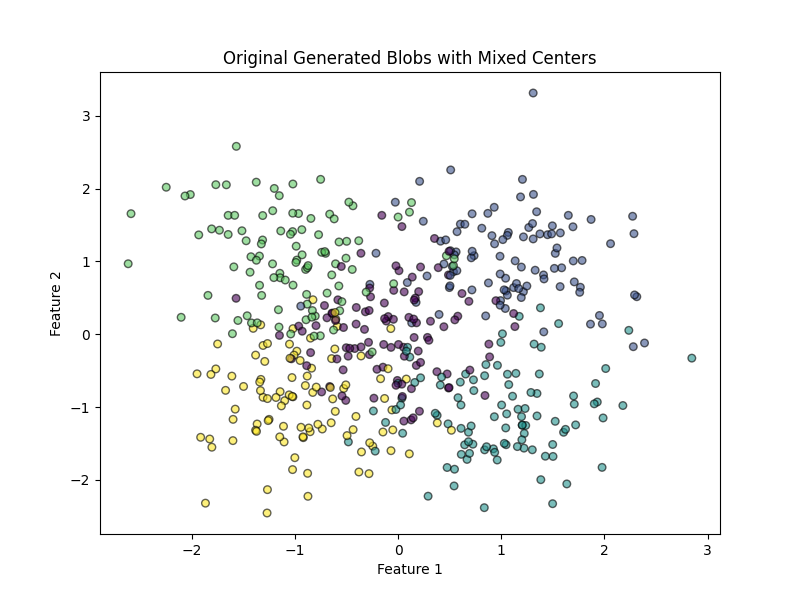
\includegraphics[width=\textwidth]{figures/eenth/original_blobs}
		\caption{Original}
		\label{fig:original}
	\end{subfigure}
	\hfill
	\begin{subfigure}[b]{0.3\textwidth}
		\centering
		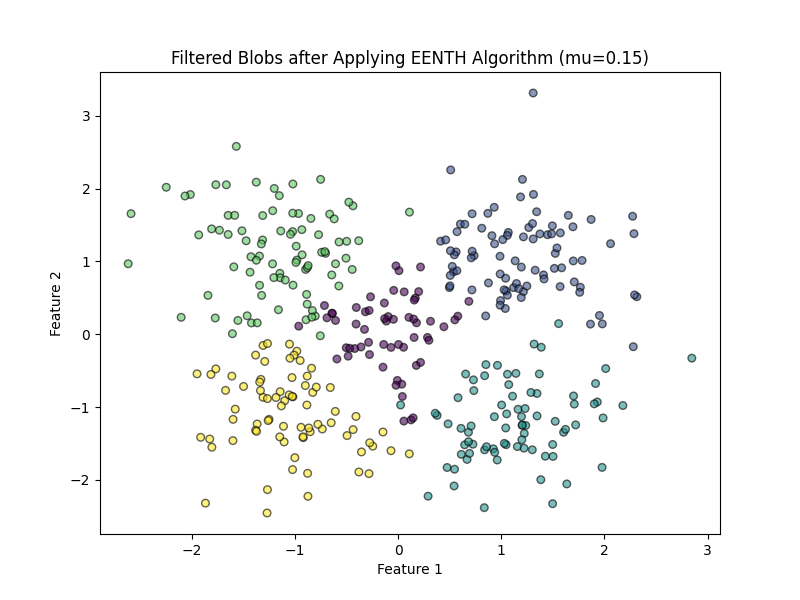
\includegraphics[width=\textwidth]{figures/eenth/filtered_blobs_mu_0.15}
		\caption{$\mu = 0.2$}
		\label{fig:mu0.2}
	\end{subfigure}
	\hfill
	\begin{subfigure}[b]{0.3\textwidth}
		\centering
		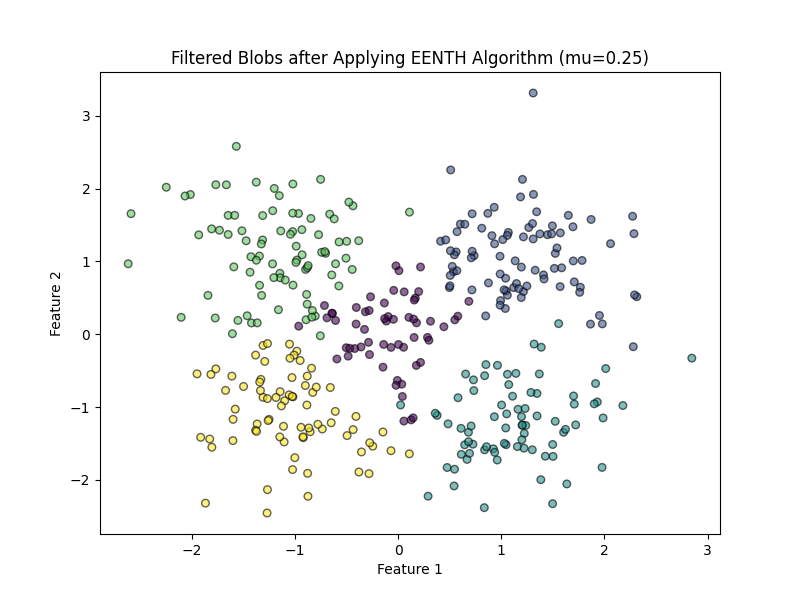
\includegraphics[width=\textwidth]{figures/eenth/filtered_blobs_mu_0.25}
		\caption{$\mu = 0.4$}
		\label{fig:mu0.4}
	\end{subfigure}
	\caption{EENTH method illustration for $\mu = 0.2$ and $\mu = 0.4$.}
	\label{fig:mu_variation_1}
\end{figure}

\begin{figure}[ht]
	\centering
	\begin{subfigure}[b]{0.3\textwidth}
		\centering
		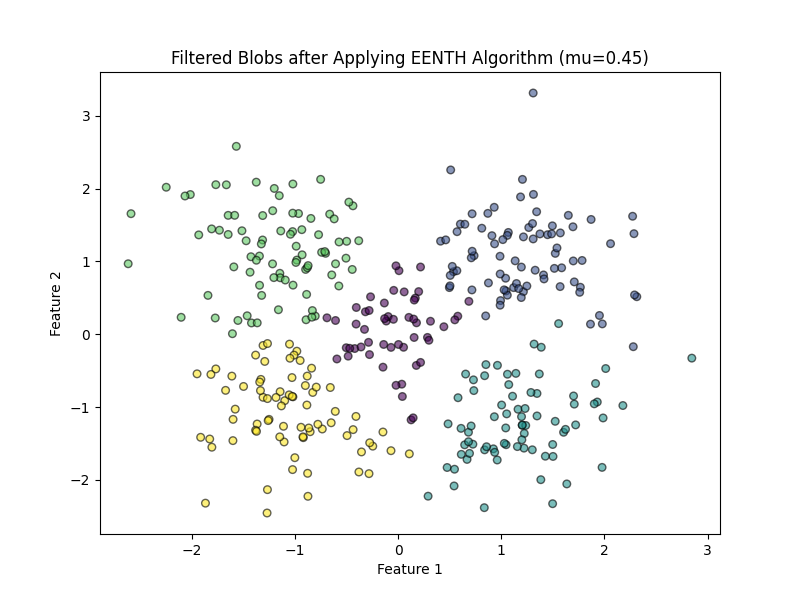
\includegraphics[width=\textwidth]{figures/eenth/filtered_blobs_mu_0.45}
		\caption{$\mu = 0.45$}
		\label{fig:mu0.45}
	\end{subfigure}
	\hfill
	\begin{subfigure}[b]{0.3\textwidth}
		\centering
		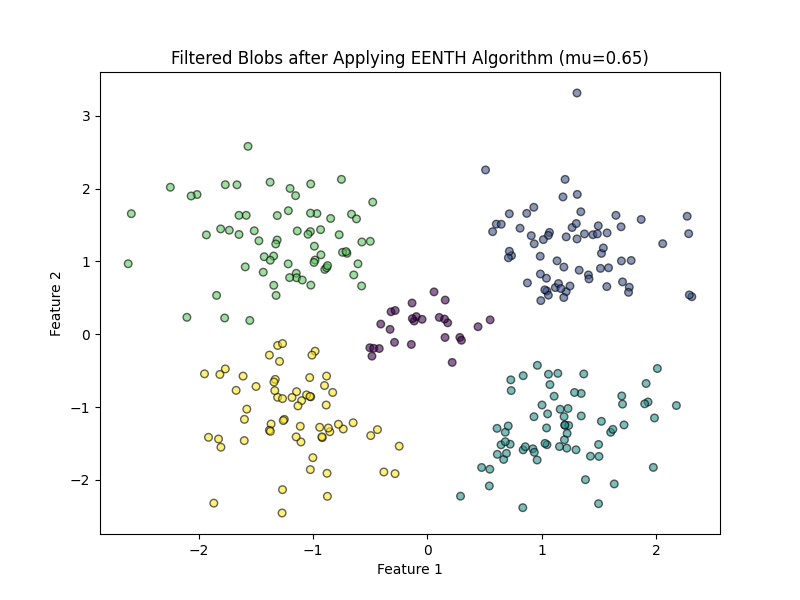
\includegraphics[width=\textwidth]{figures/eenth/filtered_blobs_mu_0.65}
		\caption{$\mu = 0.65$}
		\label{fig:mu0.65}
	\end{subfigure}
	\hfill
	\begin{subfigure}[b]{0.3\textwidth}
		\centering
		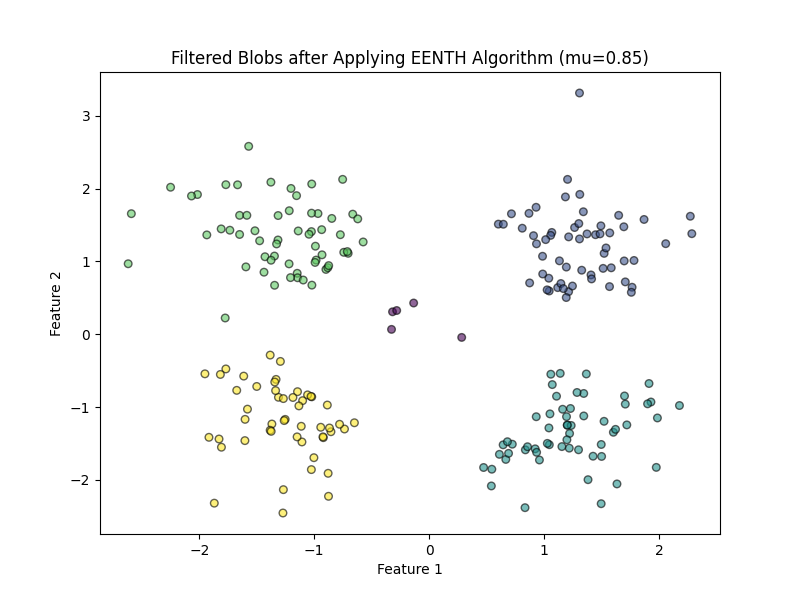
\includegraphics[width=\textwidth]{figures/eenth/filtered_blobs_mu_0.85} % Add the new plot here
		\caption{$\mu = 0.85$}
		\label{fig:85}
	\end{subfigure}
	\caption{EENTH illustration $\mu=0.45,0.65,0.85$}
	\label{fig:mu_variation_2}
\end{figure}

	

\subsubsection{DROP3}
This section covers the main concepts of the third method in the Decremental Reduction Optimization Procedure (DROP) family \cite{wilson2000reduction}. We describe the core steps and illustrate the method on $D_1$ in \textbf{Figure} \ref{fig:2dDataset}.

\begin{enumerate}
	\item \textbf{Remove Noise}: First, remove noisy instances using Edited Nearest Neighbor (EEN) \cite{wilson1972asymptotic}, where any misclassified instance by its $k$-nearest neighbors is removed. The outcome is shown in \textbf{Figure} \ref{fig:2dEEN}, with noise removed.
	
	\begin{figure}[ht]
		\centering
		\begin{minipage}{0.3\textwidth}
			\centering
			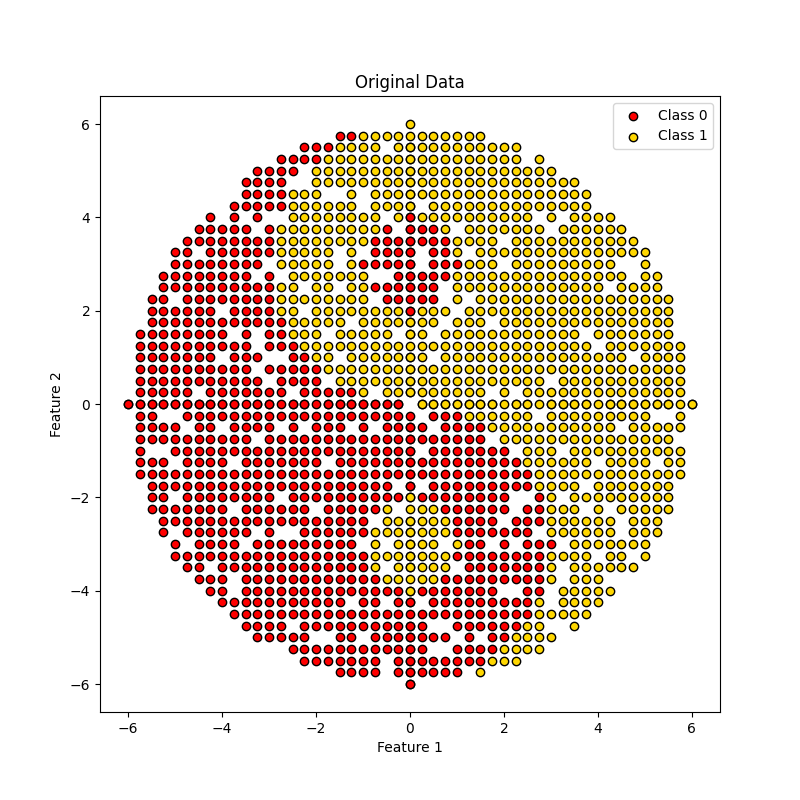
\includegraphics[width=\textwidth]{figures/DROP3/2dDataset}
			\caption{Original Dataset}
			\label{fig:2dDataset}
		\end{minipage}\hfill
		\begin{minipage}{0.3\textwidth}
			\centering
			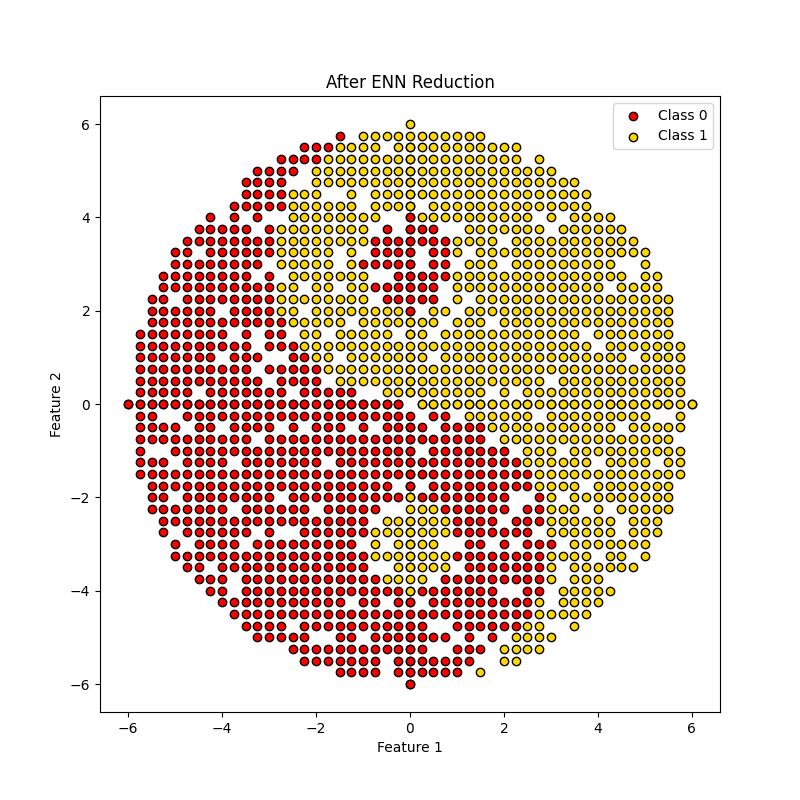
\includegraphics[width=\textwidth]{figures/DROP3/2dEEN}
			\caption{Effect of EEN}
			\label{fig:2dEEN}
		\end{minipage}\hfill
		\begin{minipage}{0.3\textwidth}
			\centering
			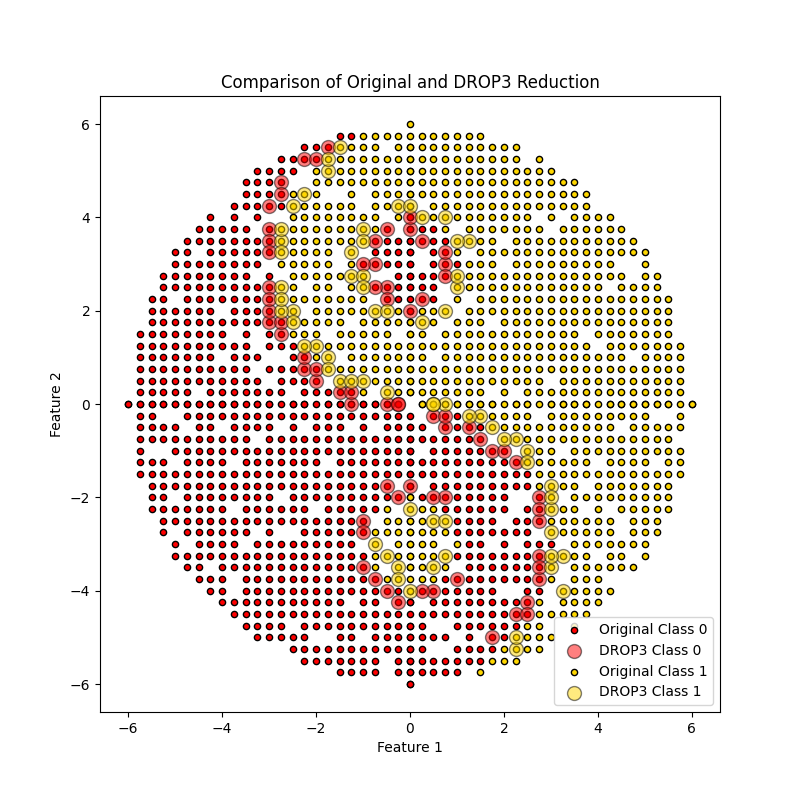
\includegraphics[width=\textwidth]{figures/DROP3/DROP3}
			\caption{Effect of DROP3}
			\label{fig:DROp3Total}
		\end{minipage}
	\end{figure}
	
	\item \textbf{Sort Points}: Next, prioritize removing points farthest from the decision boundary. For each $x_i \in S$ with class $y_i$, calculate the distance to the nearest point of a different class.
	
	\item \textbf{Delete Points}: Starting with points farthest from the boundary, check if any associated points receive more correct classifications without $x_i$ than with it. If so, remove $x_i$ from $S$.
\end{enumerate}
